In this paper, I employ a Regression Discontinuity (RD) design to examine how households' electricity consumption responds to the marginal price informed via monthly energy statements under Increasing-Block Pricing (IBP). In previous studies, a common challenge in measuring consumption responses to price changes has been discussed repeatedly: constructing a well-defined control group is difficult due to that consumers typically experience the same price variation. However, the setting I exploit in this paper enables me to address the identification challenge.  

The RD design I implement in this paper relies on three points. First, the marginal price is a step function of consumption level in the increasing block-tier rate plans chosen by SMUD residential customers. That is, under IBP, the price a household pays for the marginal electricity consumption increases discontinuously at some pre-determined aggregate consumption in a billing cycle. Second, as discussed in Section \ref{C1-Sub-Sub-section:Monthly-Bill-as-the-Only-Source-of-Electric-Usage-Information-for-Households}, before 2009, SMUD residential customers had practically no way to know the marginal price in a billing cycle within the very cycle. They were informed of the price they paid for the marginal electricity consumption in a billing cycle only through their electricity bills delivered in the following cycle. Third, it is not generally feasible for households to consume only a pre-targeted amount of electricity within a billing cycle. In general, households have limited capability to control their electricity consumption due to the minimal essential demand (e.g., usage for refrigerators and lighting). In addition, because household electricity consumption heavily depends on outdoor temperature variation, managing one's own electricity usage not to exceed the target amount of electricity consumption could incur too high information cost, which might result in rational inattention \citep{Rational-Inattention-and-Energy-Efficiency_Sallee_(2014)}, even if households are available to adjust their consumption behavior with complete flexibility. 

\afterpage{
    \begin{figure}[t!]
        \centering
        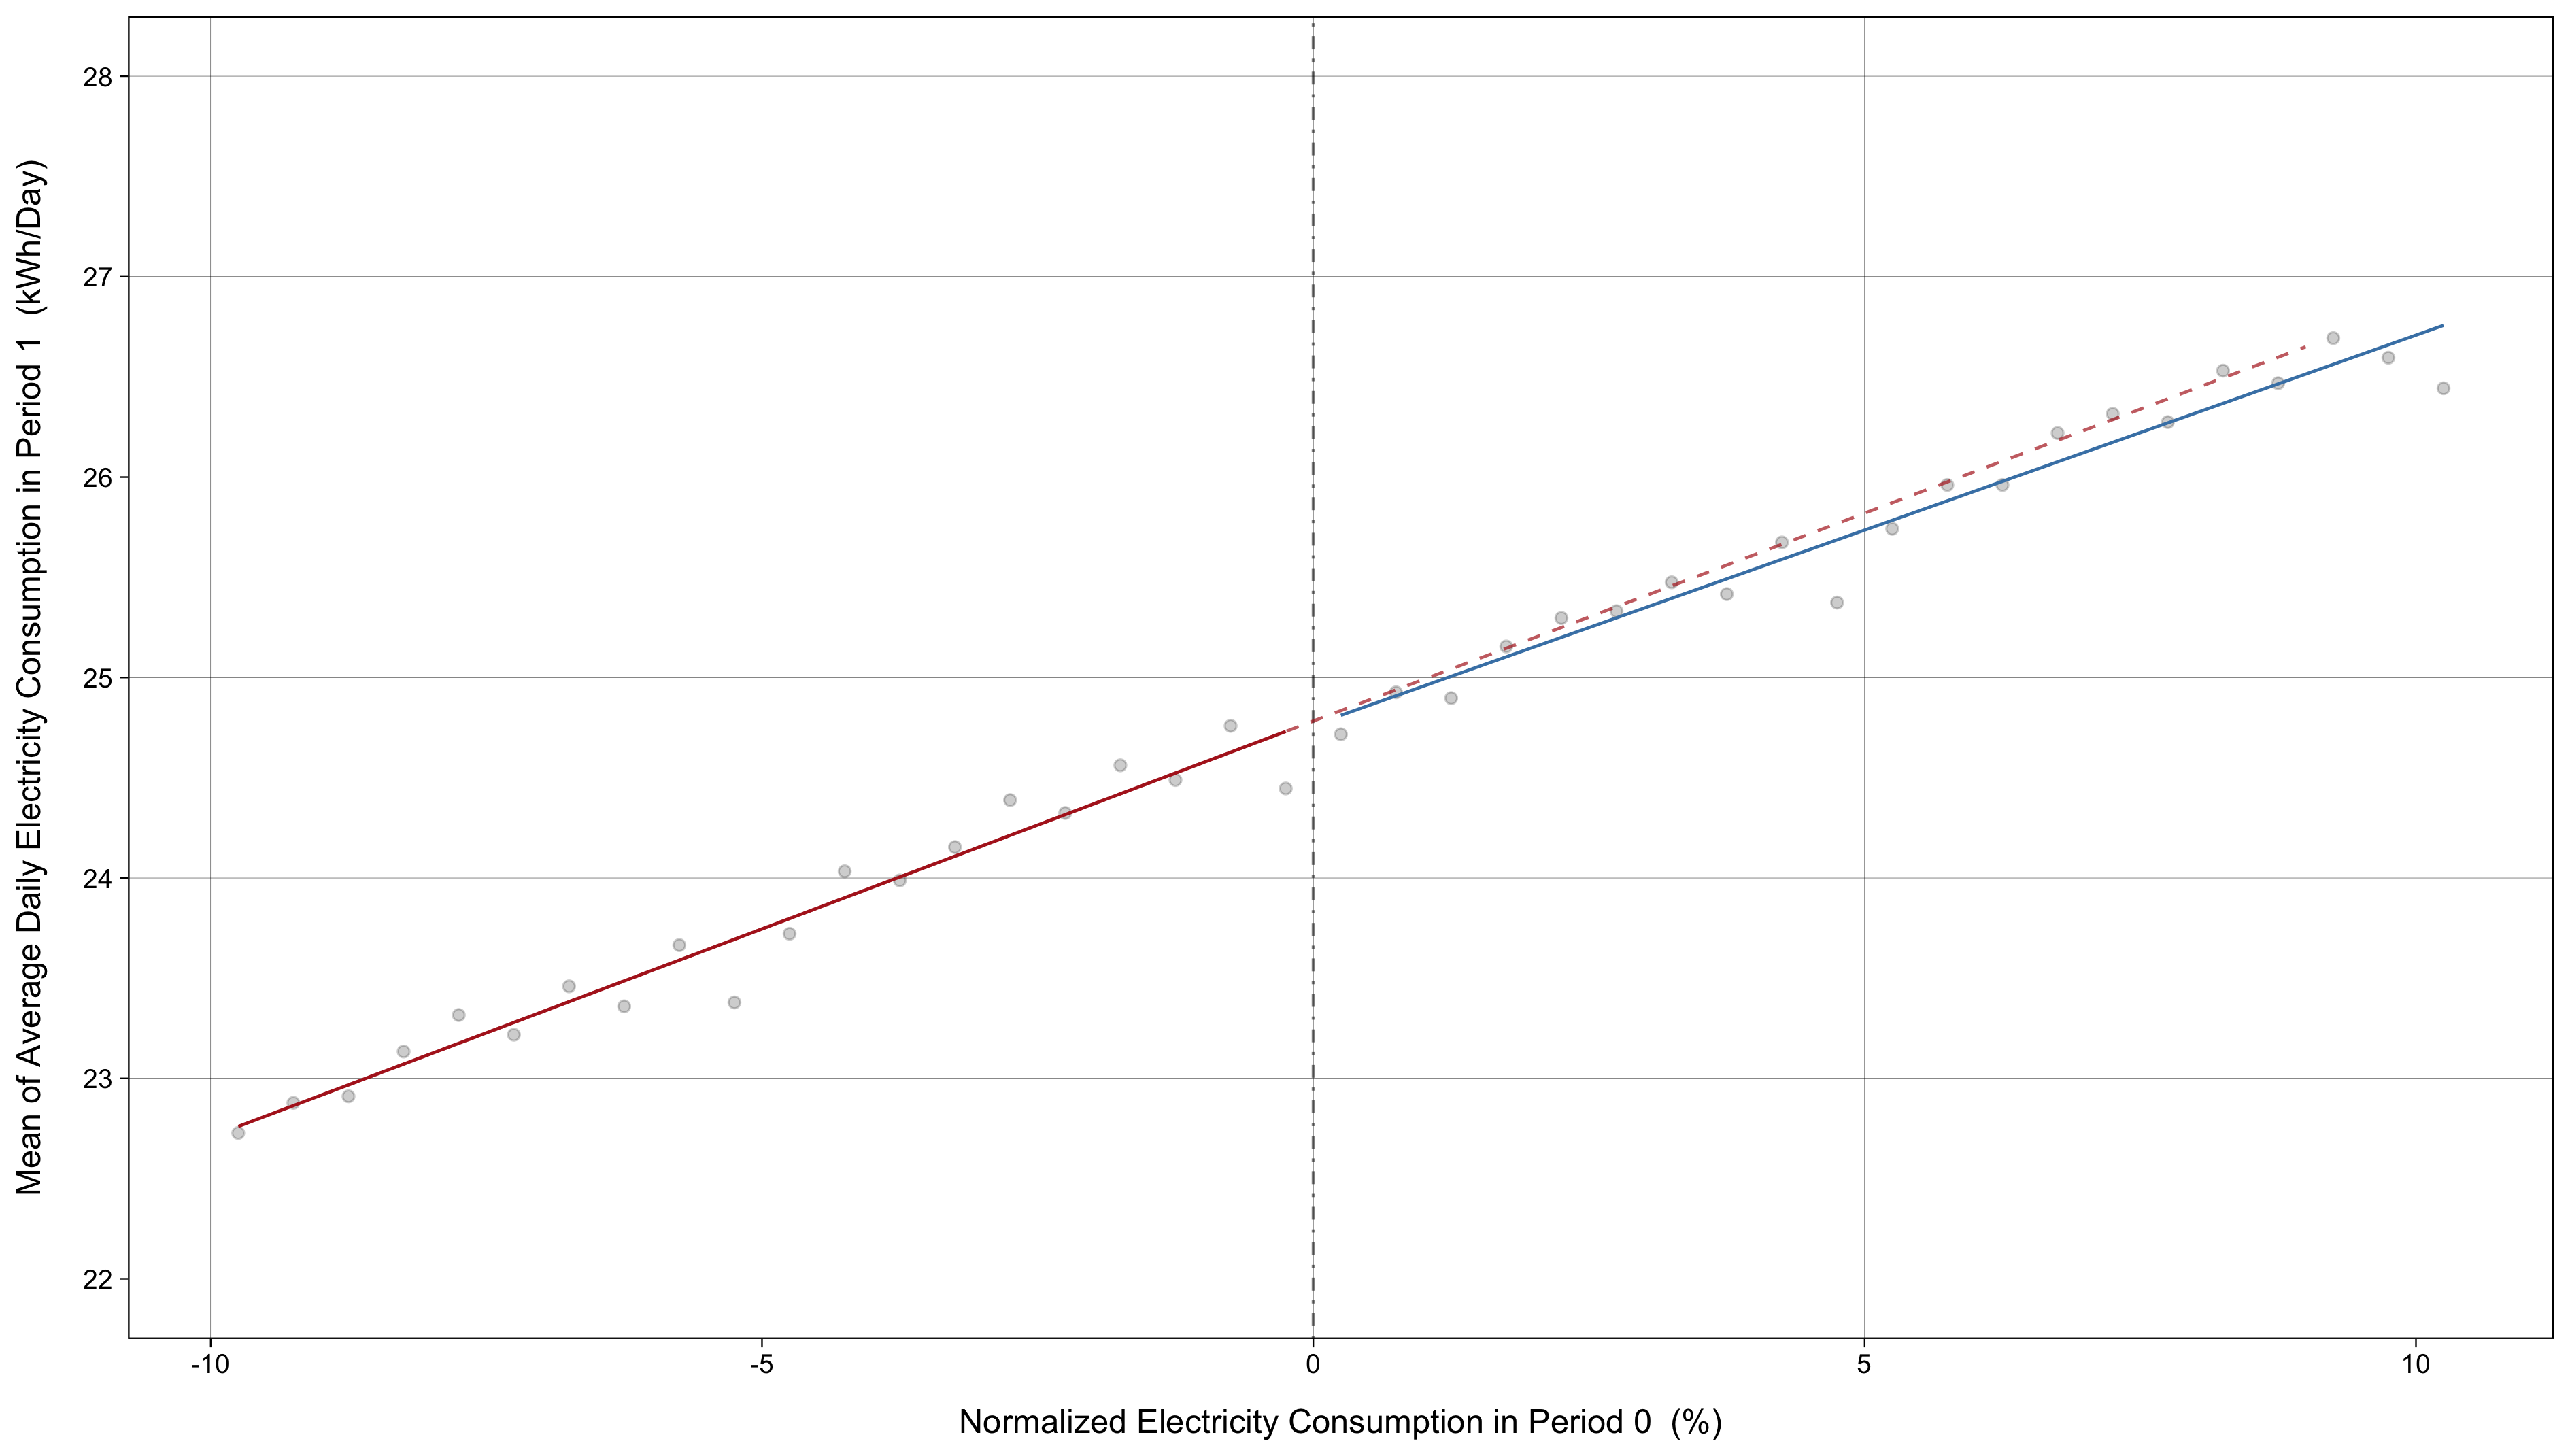
\includegraphics[scale = 0.115]{02_Chapter-1/00A_Figures/Figure_Average-Daily-Electricity-Consumption-in-Period-1-over-NC0.png}
        \caption{Mean of Average Daily Electricity Consumption in Period 1 over $\overline{NC}_{0}$}
        \caption*{
            {\small
            \textit{Note}: 
            This figure's scatter points correspond to the average daily electricity consumption in Period 1, computed by bins with a bandwidth of 1\% of $\overline{NC}_{0}$. The solid line on each side of the vertical dot-dash line is a parametric fit obtained from the regression of the average daily electricity consumption on $\overline{NC}_{0}$. The dashed red line is an extension of the solid red line. The gap between the dashed red and solid blue lines seems to indicate a non-negligible treatment effect. 
        }}
        \label{Figure:Average-Daily-Electricity-Consumption-in-Period-1-over-NC0}
    \end{figure}
}
Regarding the first point, the discontinuities under the nonlinear electricity schedules allow utilizing a RD design. In my RD design, the running variable is the level of electricity consumption in a household during a billing period (denoted as Period 0), whereas the outcome variable corresponds to the household's average daily electricity consumption during the subsequent billing period (denoted as Period 1). So, in this quasi-experimental setting, I compare SMUD residential customers just above and below the thresholds of the tier rates, called base usage quantities. Under IBP, surpassing a threshold leads to an increase in the marginal price households pay for electricity consumption mechanically. Here, the discontinuous increase in the marginal price, which accompanies \textit{no discontinuous change in the average price}, applies only to Period 0, not to Period 1.\footnote{The average price smoothly grows around the cutoff point.} Moreover, information about whether households were subject to a higher marginal price in a billing period is delivered early in the subsequent billing period through their monthly electricity bills. Therefore, any changes with respect to the electricity consumption of households just above the threshold (i.e., households in the treatment group) in Period 1, compared to households just below the threshold (i.e., households in the control group), can be understood as their short-term behavioral responses stemming from the sharp jump in the marginal price in Period 0. Figure \ref{Figure:Average-Daily-Electricity-Consumption-in-Period-1-over-NC0}, showing how the mean of households' average daily electricity consumption in Period 1 evolves around the lower base usage quantity, seems to indicate the existence of such behavioral responses. 

The last two points demonstrate that the fundamental identifying assumption of the RD design is reasonable. The fundamental identifying assumption is that SMUD residential customers just below a base usage quantity are expected to be very similar to those just above it, along with observed and unobserved characteristics. In other words, a group of households in the small neighborhood of the threshold is not different from one obtained from a randomized experiment. In my setting for empirical analysis, SMUD residential customers were unable to be aware of how far away they were from a given cutoff point in real time. Furthermore, as discussed above, it is not convincing that they can perfectly control their electricity consumption during a billing cycle to use exactly a target amount of electricity by the end of the last day of the billing cycle. Hence, it is highly unlikely that the customers precisely adjusted their consumption behavior so as to avoid surpassing the cutoff point, which in turn prevented them from leading to a higher marginal price. That is, it seems plausible that households were not able to sort themselves around the threshold strategically. Therefore, any discontinuity gap in the outcome variable can be attributed to the discontinuous increase in the marginal price at the threshold in Period 0. 
